% To submit for peer review comment the maketitle command.
\documentclass[man,natbib,floatsintext]{apa6}


\usepackage[utf8]{inputenc}
\usepackage{array}
\usepackage{booktabs}
\usepackage{capt-of}
\usepackage{adjustbox}
\usepackage{rotating}
\usepackage{graphicx}
\usepackage{subcaption}
\usepackage{fancyvrb}
\usepackage{setspace}
\usepackage{dcolumn}
\usepackage[longnamesfirst]{natbib}
\usepackage{float}
\usepackage[toc, page]{appendix}
\usepackage{placeins}
\usepackage{outlines}
\usepackage[justification=centering]{caption}
\usepackage{tabularx}
\usepackage{booktabs}
\usepackage{longtable}
\usepackage{array}
\usepackage{multirow}
\usepackage{wrapfig}
\usepackage{float}
\usepackage{colortbl}
\usepackage{pdflscape}
\usepackage{tabu}
\usepackage{threeparttable}
\usepackage{threeparttablex}
\usepackage[normalem]{ulem}
\usepackage{makecell}
\usepackage{xcolor}
\usepackage{amsmath}
\usepackage{pgfplots}
\pgfplotsset{compat = newest}
\usetikzlibrary{positioning, arrows.meta}
\usepgfplotslibrary{fillbetween}
\usepackage{titlesec}
\usepackage{tikz}
\usepackage{pgfplots}
\usepackage{graphicx}
\usepackage{nicematrix}
\usepackage[table, dvipsnames]{xcolor}
\allowdisplaybreaks
\usepackage{threeparttable}


\pagenumbering{gobble}
\graphicspath{ {./images/} }
\title{\textbf{The Effect of ESG Ratings on Asset Returns
} }
\shorttitle{ESG Rating \& Asset Returns}

\author{Lucas Moura Bender,
Steven Agen,
Yui Kan Kong,
Frank Zhu,
Konstantine Jalagonia
}

\affiliation{ \\ \\ Group E2\\ Applied Statistics and Econometrics I \\ New York University}

\note{Dec 17, 2022}

\keywords{ESG,Fama-French 3 factor
}

\authornote{ Our thanks to Professor Nandi and Dragos Ailoae for their help in guiding us on this paper and for all of their support throughout the semester. This paper is dedicated to them.  
}

\date{December 17, 2022}

\begin{document}


\bibliographystyle{plainnat}

\maketitle


% Do not move setcounter earlier or the abstract will be numbered too
\setcounter{secnumdepth}{3}
\setcounter{tocdepth}{3}

\section{\textbf{Introduction}}
\pagenumbering{arabic}
ESG investing, as defined by \citet{msci_2022}, is “the consideration of environmental, social and governance factors alongside financial factors in the investment decision-making process.” ESG can be thought of as a set of standards which investors can use to "judge" companies or investments. While the basis of ESG is fundamentally a qualitative measure, several companies have ascribed "ESG ratings" or "scores" as a way to provide a quantitative measure of ESG factors with respect to specific firms. Individual companies are assigned an ESG score which evaluates how these firms "perform" with key ESG factors. The foundations of these ratings can be broken down further.

Carbon emissions, air and water pollution, energy efficiency, climate policies, and other sustainability factors pertain to the "Environment" side of ESG. The "Social" aspects of ESG will be a value of how companies interact with “internal” and “external” stakeholders. Factors such as a company’s human rights record, their labor standards or even customer satisfaction can play a role. Lastly, the "Governance" side of ESG will be a measure of diversity, transparency, accountability, and integrity of a company and its structure.
In order to assess whether ESG ratings can have any significant impact on asset returns, this paper will first explore whether, in theory, investors are at all concerned with ESG or ESG ratings. Indeed, ESG as a concept has seen an increase in popularity in recent years. Many financial institutions such as brokerage firms are now offering financial services with "ESG considerations" at the forefront. Companies such as Ernst \& Young (EY) advertise services with "Sustainability and ESG" in mind, and others, such as Betterment, even offer financial instruments, such as ETFs, geared towards an "ESG investor" \citep{EY}. It would stand to reason then that many mainstream investors are indeed attentive to ESG measures.

While it seems likely that ESG matters to some investors, it is not clear how much it matters, or if indeed it matters to a large enough number of investors as to make any impact significant. It could be the case, for example, that while some investors may be willing to pay a premium for more socially responsible firms, other investors might find attractive the environmentally unsustainable practices that could lead to higher profit margins. Consider the oil industry, for example, where companies may deliver a higher return on investment, even though it would be expected that they would have a lower ESG score compared to those not in the energy sector. It is difficult to conclude, prima facie, from the outset whether ESG will have a significant impact on asset returns.



\section{\textbf{Literature Review}}
Some economists have tried to insert ESG data into existing finance models. A study from the Kenan Institute modeled how investors are willing to place a higher valuation on companies with strong ESG scores, leading to a convergence among other companies in the market towards high ESG performance. However, no evidence is presented in this paper and the author suggests that empirical research will be difficult to conduct due to the nature of the relationship between stock returns and ESG. Empirical research has focused on two approaches: one of them is research on the correlation of ESG news and stock price, and another method was conducted based on a survey.
  
\citet{capelle-blancard_petit_2017} tested for correlation between stock prices and media exposures or press releases. They found stock prices correlate to the former but not the latter. \citep{philip} suggests how stock prices are affected by corporate social responsibility. These are some of the examples of research via ESG news. The problem with this kind of research suggested by Krugger was that it is difficult to explicate precisely the relations between ESG news and returns. A possible explanation is that investors focus only on returns and the ESG factor was one of the indicators of returns. This thought was confirmed by \citep{aaron_yoon} as their research found that stock prices only correlated with ESG news, and stock prices are the variable containing return information in them. Another paper by \citep{ashwin} suggests that a high ESG rating reduces risk, which is another factor affecting stock price so ESG affects pricing in an indirect way.
  
The latter type of research usually is conducted via surveys sent to institutional investors and evidence from these suggests that investors may be willing to pay a 10\% premium or more for equity in those companies. The problem, again, was that no empirical evidence existed to support the claim. 



\section{\textbf{Data and Methodology}}

The data in this paper is obtained from the Wharton Research Data Services (WRDS), where a consortium of data providers was hosted. Our analysis drew a random sample of 1276 firms (US Equity only) for our cross-sectional analysis, and the corresponding variables of interest in the year 2021 were queried from the WRDS data providers. Firm-level financial data, including company returns, market capitalization, and various financial ratios were collected from the CRSP database. Firm-level Fama-French Betas were provided by the WRDS Beta Suite. Finally, the S\&P ESG score associated with each company, including its dimensional scores, was downloaded from the S\&P Global Database.


\subsection{\textbf{Variables}}

The descriptive statistics (Table 1) summarizes the characteristics associated with each of the variables used in the forthcoming analysis. It should be noted that since the data are queried from different providers, the availability of data across the variables differs slightly. The analysis undertaken thenceforth is done with complete observations only. In addition, to adhere to the cross-sectional requirement of this project, the continuous variables such as market capitalization, book-to-market ratio, and ESG Scores are calculated to be the average value for the given year. 

\subsubsection{{Independent variables}} \hfill\\


Market Cap: The average market capitalization of the company in the year 2021. It is defined as the average market price per share multiplied by the average total number of outstanding shares. This variable is also the proxy through which the company's size effect is measured. Research has suggested that a firm's market capitalization is inversely related to its returns \citep{banz_1981, fama_french_1993}.

Book to Market: The book-to-market ratio is calculated as the firm's book value (tangible assets minus liabilities and preferred shares) divided by its market value, and the ratio is then averaged over the year 2021. It is the proxy through which the company's value effect is measured. \citet{stattman2020, fama_french_1993} have found that the book-to-market ratio is positively correlated with the company's return. 

Shares Turnover: The company's average shares turnover ratio in 2021. It is calculated from shares traded (trade volume) divided by shares outstanding. Previous research suggests that share turnover is negatively correlated with returns, and its effect was significant even after controlling for a firm's size effect and value effect \citep{lee_swaminathan_2000}. 

Accrual: The company's average change in accruals (net working capital less depreciation) in 2021. Studies have suggested that there exists a strong negative relationship between accrual and company returns, after controlling for the size and value effect of the company \citep{richardson_sloan_soliman_tuna_2005}.

Fama-French Market Beta: Market Beta used in our model is downloaded from WRDS Beta Suite based on the Fama-French 3-factor model. This variable represents the company's sensitivity or co-movement with the overall market, and it's often used to control for the impact of broader market changes on company-level returns (WRDS Beta Suite). 

S\&P Global ESG Score: The cumulative S\&P Global's ESG rating for a given company. This score examines the company's leadership in reading with its employees and the communities where the company operates. It is a continuous variable that is a weighted summation of scores across three dimensions: Environment, Social, and Governance. The specific criteria that the score measures include are climate strategy, environmental reporting, biodiversity, corporate philanthropy, and labor practice. 

Industries: This is a categorical variable that indicates the sector in which the firms are operating. In total, there are eleven industries in our sample, from consumer discretionary to Energy; Basic Materials is the base category for our analysis. Financial services are the most represented at 22\%, and utilities are the least represented at 7\%. 

\subsubsection{{Dependent variable}}

Company excess return is defined as the company's cumulative return in 2021 less the risk-free rate of the year. Following the broader literature, the risk-free rate is chosen to be the 10-year yield on US Treasury. This return represents a company's return in excess of the rate of return of an investment that carries zero risk. 


\subsection{\textbf{The Model}}
The model used in this paper is inspired by and based on the Fama–French three-factor model. The Fama-French three-factor model is an asset pricing model that expands on the original Capital Asset Pricing Model (CAPM), taking into account the impact of size effect and a value effect on asset returns. This model stems from the empirical observation of the stock market, where smaller firms tend to outperform larger companies, and those with a higher book-to-market ratio would outperform those with a lower ratio (Fama and French, 1993). Specifically, the Fama-French OLS regression model specification is as follows: 
\begin{align}
&R_i-R_F=\alpha_i+\beta_i(R_M-R_F)+s_iSMB+h_iHML+ e_i  \\
&  \text{Where: } \notag \\
& R_i = \text{return of the given portfolio} \notag \\ 
&  R_F= \text{risk-free interest rate (US 10 year treasury)} \notag \\ 
&  R_M- R_F= \text{return spread between capitalization-weight stock market and cash } \notag \\ 
&  SMB = \text{the return spread of small minus large stocks (the size effect)} \notag \\ 
&  HML= \text{return spread of cheap minus expensive stocks (the value effect) } \notag 
\end{align}
The Fama-French three-factor model has been widely regarded as the gold standard in asset pricing. However, the parameters set forth in this paper require that the analysis be conducted in a cross-sectional context. To meet these restrictions, the model used in this paper will adapt the Fama-French 3-factor model (1) and make it a cross-sectional model. Specifically, our empirical model uses firm-specific financial ratios as a proxy to account for the factors presented in Fama-French, with additional variables that carry explanatory power toward asset returns as suggested by the broader literature. The base OLS regression model used in this paper is as follows: 
\begin{align}
&R_i-R_F =\alpha_0+\beta_1 FFB +\beta_2 MC + \beta_3 BM + e_i \\
&  \text{Where: } \notag\\
& R_i-R_F = \text{Company Excess Return}\notag \\ 
&  FFB = \text{Fama-French Betas} \notag \\
&  MC = \text{Market Capitalization} \notag \\
&  BM= \text{Book-to-market ratio} \notag 
\end{align}
Note that the second factor, the firm’s market capitalization, accounts for the firm's size effect on stock returns, and it is a proxy for the $SMB$ factor in the original Fama-French model (1). On the other hand, the third factor, the Book to Market ratio, accounts for the value premium in returns, replicating the $HML$ factor. The $FFB$ factor --- the actual market Beta variable from Fama and French’s results obtained via WRDS --- represents the co-movement of company-specific returns to market returns, and its inclusion controls for the sensitivity of individual stocks to the overall market. 
After this base model, a second OLS can be established, this time with ESG score as a factor:
\begin{align}
&R_i-R_F =\alpha_0+\beta_1 FFB +\beta_2 MC + \beta_3 BM +\beta_4 ESG + e_i \\
&  \text{Where: } \notag\\
&  ESG = \text{S\&P Global Composite ESG Score} \notag 
\end{align}
In order to make a more sophisticated model, which could account for more variations in return, a third OLS was created, adding two more variables that have demonstrated impact on asset returns in various studies, Shares Turnover Ratio, and Accruals.
\begin{align}
&R_i-R_F =\alpha_0+\beta_1 FFB +\beta_2 MC +\beta_3 BM + \beta_4 ESG +\beta_5 ST + \beta_6 ACC + e_i \\
&  \text{Where: } \notag\\
&  ST= \text{Shares Turnover ratio } \notag \\ 
&  ACC = \text{Accruals} \notag 
\end{align}
Lastly, a 4th and final OLS is derived, which includes a set of industry dummy variables to control for industry-specific effects. This fourth regression will include 10 dummy variables, in order to account for a total of 11 different industries.
\begin{align}
R_i-R_F =&\alpha_0+\beta_1 FFB +\beta_2 MC +\beta_3 BM + \\
          &+\beta_4 ESG +\beta_5 ST + \beta_6 ACC +\beta_7 IND + e_i\notag \\
  &\text{Where: } \notag\\
  &IND= \text{Industry} \notag 
\end{align}
With these 4 models, it is then possible to test whether the ESG scores, have any effect on asset returns. Our analysis is conducted under the null hypothesis that ESG scores have no statistically significant impact on asset returns. The Alternative Hypothesis will be that ESG scores have a statistically significant impact on asset returns. To test for the possible issue of multicollinearity, the General Variance Inflation Factors (GVIF) are calculated and used instead of Variance Inflation Factors because the model included the categorical variable $Industry$. The result of the test is presented in Table 2, and since the maximum GVIF in our model does not exceed the threshold, there is low multicollinearity in the model. 


\section{\textbf{Results}}

It is important to note before any results can be interpreted, that there already exists an expectation that the R-Squared values for the regressions on the cross-sectional models are going to be fairly low. This finding is in line with relevant academic research where R Squared is around 0.01 \citep{fama_french_1993}. There are a few reasons for these expectations, the main one being that the original Fama-French model (1) is set in a different context than the cross-sectional models (2),(3),(4), and (5) for this paper. Fama and French were able to control for changes in a company’s or a portfolio’s time trend effects, something that was not possible in a cross-sectional setting. As noted previously, the Fama-French model (1) relied on diversified portfolios, which mitigates unsystematic risk, therefore, there should be less ‘unexplained’ variance. In the cross-sectional models (2-5) this is not something that can be accounted for. It was not possible to use diversified portfolios in this analysis given that ESG data collection only began recently and that scores do not update often. The Fama-French model was primarily applied to well-diversified portfolios to avoid introducing the effect of firm-specific risk in the analysis that would bias the results.

The regression results are shown in Table 3. The first regression includes only the factor carried over from the original Fama-French 3-factor model (1), which has the following regression equation:
$$R_i-R_F =\alpha_0+\beta_1 FFB+\beta_2 MC+\beta_3 BM+ e_i$$
All of the coefficients from this regression are statistically significant at a 10\% significant level, with the coefficients for Book to Market ratio and the Market Betas being significant at a 5\% level. For the most part, these results align with expectations from economic research. The market beta has a positive coefficient, which is aligned with the theory behind CAPM and the Fama-French original model's assumption that stocks will require a higher return if they are more volatile compared to the market portfolio. Additionally, Fama and French suggest that value stocks will outperform growth stocks. The positive, statistically significant, coefficient on the B/M ratio suggests that this expectation holds. 

One coefficient was not in line with expectations, however, and that was the coefficient on market capitalization. Fama and French suggest that there exists a “small firm effect” in which small firms with low market capitalization tend to outperform larger firms. However, the positive coefficient from Regression 1 in Table 3 suggests this is not the case. One explanation for this is that ESG data is for the most part available only for bigger firms, which will have high market capitalization. As the coefficient is close to zero, and not statistically significant at the 5\% level, it is not economically significant. Overall, our adapted, cross-sectional regression model (1) still exhibits roughly the same result as the underlying Fama-French model. 
For the second regression with the added ESG score:
$$R_i-R_F =\alpha_0+\beta_1 FFB+\beta_2 MC+\beta_3 BM+ beta_4 ESG+e_i$$
In contrast to regression (1) from Table 3, for regression(2) there is less unexplained return, as the R-square value increased. The coefficient on ESG scores suggests a positive correlation between ESG and asset returns, which is significant at a 5\% level. This  correlation is an indicator that ESG scores will indeed have a positive impact on returns, however, it is still not in keeping with expectations that there is a positive, insignificant, coefficient on market capitalization. 
In order to address the considerably low R-squared value for Regression (2), Regression (3) was run: 
$$R_i-R_F =\alpha_0+\beta_1 FFB +\beta_2 MC +\beta_3 BM + \beta_4 ESG +\beta_5 ST + \beta_6 ACC + e_i $$
With the introduction of the new relevant variables--- shares turnover and accrual, there is an increase in R square, while the coefficient of ESG scores remains positive and statistically significant. In fact, the magnitude of the coefficient on ESG increased in Regression (3) as compared to Regression (2). The coefficient on Market Cap does indeed now have a negative, though still insignificant, coefficient which more closely resembles the model assumptions. 
Finally, as mentioned in the introduction, returns can vary by industry, so it is important to account for these variations. In order to do this, the industry is included as a dummy variable in Regression (4):
$$R_i-R_F =\alpha_0+\beta_1 FFB +\beta_2 MC +\beta_3 BM + \beta_4 ESG +\beta_5 ST + \beta_6 ACC +\beta_7 IND +  e_i $$

 The R-squared value for Regression (4) increased to 0.12033, most of the other results, however, are similar to the previous regression (3) with shares turnover and accrual, in line with previous studies, being statistically significant. Fama and French in their 1992 paper \cite{Fama_french_1992} found that R-squared tends to be significantly lower when using a cross-sectional model compared to a time-series setting. Other authors have reproduced the same result. The reason for this is that the high predictive power of the asset pricing models comes from the time trend in stock returns. Since it is not possible to account for the historical returns and autoregressive dynamics of the model in a cross-sectional setting, the predictive power that other asset pricing models have is lost.


The main coefficient of interest, ESG score, maintained a high significance throughout multiple different regressions. For regression (4), the final regression, the coefficient on ESG scores suggests a 1-point increase in ESG score is associated with a .2\% increase in return, which is economically significant. Therefore, it can be concluded there is a positive correlation between ESG scores and the return on investment.
As for heteroscedasticity and autocorrelation, autocorrelation was non-existent by assumption as time-series data was not being used. For heteroscedasticity, the Breusch-Pagan test was conducted. The p-value for the test is approximately zero suggesting that heteroscedasticity is present in our analysis. To account for this, it was necessary to use heteroscedasticity-robust standard errors in all the regressions.


\section{\textbf{Conclusion}}
Our final regression result suggests that there is a positive correlation between asset return and ESG scores. The statistically significant relationship persisted even as more control variables or individual segments of ESG were added. It would be a stretch to suggest any causal relationship or to posit the reasoning behind the relationship with given that we did not undertake a time-series regression. However, the result here still shows evidence of the strong relations between socially responsible business practices and firm returns, which would merit further exploration. Our findings have several policy implications. Since the ESG score and its individual components seem to be related to stock returns, asset managers can use the ESG score as a factor in the asset pricing model to improve the predictive power of their model and make their portfolios more sustainable. A natural first step would be to repeat the analysis in a time series context, allowing us to preserve more of the Fama-French model. Additionally, it would be interesting to see the effect of each individual factor comprising ESG on asset returns. 

Our results suffered from some constraints, including the time series data limitation which forced us to adapt the underlying base model we used. Another constraint is embedded in the nature of the ESG data. These scores are both relatively new and they are also rarely updated. We used the highest frequency, and oldest data set we could find and even then, we have less than ten years of data which only updates quarterly. In the future, we hope a better ESG data set will emerge with broader coverage.










% references
\begin{singlespace}
\bibliography{citations.bib}
\end{singlespace}
\newpage

\section{Tables}
%% Table created by stargazer v.5.2.3 by Marek Hlavac, Social Policy Institute. E-mail: marek.hlavac at gmail.com
% Date and time: Tue, Dec 06, 2022 - 23:53:40
\begin{table}[!htbp] \centering 
  \caption{ESG Regression Analysis (2021)} 
  \label{} 
    \scalebox{0.7}{
\begin{tabular}{@{\extracolsep{5pt}}lccc} 
\\[-1.8ex]\hline 
\hline \\[-1.8ex] 
 & \multicolumn{3}{c}{\textit{Dependent variable:}} \\ 
\cline{2-4} 
\\[-1.8ex] & \multicolumn{3}{c}{yearly\_return} \\ 
\\[-1.8ex] & (1) & (2) & (3)\\ 
\hline \\[-1.8ex] 
 mktcap & 0.000 & 0.000 & 0.000 \\ 
  & (0.000) & (0.000) & (0.000) \\ 
  & & & \\ 
 book\_to\_market1 & 0.097$^{***}$ & 0.056$^{**}$ & 0.056$^{**}$ \\ 
  & (0.025) & (0.027) & (0.027) \\ 
  & & & \\ 
 b\_mkt\_fama\_french\_3fac1 & 0.0004$^{***}$ & 0.0004$^{***}$ & 0.0004$^{***}$ \\ 
  & (0.0001) & (0.0001) & (0.0001) \\ 
  & & & \\ 
 SPGlobalESGScore & 0.002$^{*}$ & $-$0.00004 & $-$0.00004 \\ 
  & (0.001) & (0.005) & (0.005) \\ 
  & & & \\ 
 SPGlobalESGScore:icb\_industry\_codeCONDIS &  & 0.001 & 0.001 \\ 
  &  & (0.005) & (0.005) \\ 
  & & & \\ 
 SPGlobalESGScore:icb\_industry\_codeCONSTAP &  & $-$0.011 & $-$0.011 \\ 
  &  & (0.014) & (0.014) \\ 
  & & & \\ 
 SPGlobalESGScore:icb\_industry\_codeENERGY &  & 0.011$^{**}$ & 0.011$^{**}$ \\ 
  &  & (0.005) & (0.005) \\ 
  & & & \\ 
 SPGlobalESGScore:icb\_industry\_codeFINL &  & 0.003 & 0.003 \\ 
  &  & (0.005) & (0.005) \\ 
  & & & \\ 
 SPGlobalESGScore:icb\_industry\_codeHEALTH &  & $-$0.0003 & $-$0.0003 \\ 
  &  & (0.006) & (0.006) \\ 
  & & & \\ 
 SPGlobalESGScore:icb\_industry\_codeINDL &  & $-$0.0001 & $-$0.0001 \\ 
  &  & (0.005) & (0.005) \\ 
  & & & \\ 
 SPGlobalESGScore:icb\_industry\_codeREIT &  & $-$0.003 & $-$0.003 \\ 
  &  & (0.006) & (0.006) \\ 
  & & & \\ 
 SPGlobalESGScore:icb\_industry\_codeTECH &  & 0.001 & 0.001 \\ 
  &  & (0.005) & (0.005) \\ 
  & & & \\ 
 SPGlobalESGScore:icb\_industry\_codeTELECOM &  & $-$0.002 & $-$0.002 \\ 
  &  & (0.006) & (0.006) \\ 
  & & & \\ 
 SPGlobalESGScore:icb\_industry\_codeUTIL &  & 0.002 & 0.002 \\ 
  &  & (0.006) & (0.006) \\ 
  & & & \\ 
 Constant & 0.147$^{***}$ & 0.179$^{***}$ & 0.179$^{***}$ \\ 
  & (0.036) & (0.036) & (0.036) \\ 
  & & & \\ 
\hline \\[-1.8ex] 
Observations & 1,023 & 1,023 & 1,023 \\ 
R$^{2}$ & 0.025 & 0.060 & 0.060 \\ 
Adjusted R$^{2}$ & 0.021 & 0.047 & 0.047 \\ 
Residual Std. Error & 0.466 (df = 1018) & 0.460 (df = 1008) & 0.460 (df = 1008) \\ 
F Statistic & 6.423$^{***}$ (df = 4; 1018) & 4.619$^{***}$ (df = 14; 1008) & 4.619$^{***}$ (df = 14; 1008) \\ 
\hline 
\hline \\[-1.8ex] 
\textit{Note:}  & \multicolumn{3}{r}{$^{*}$p$<$0.1; $^{**}$p$<$0.05; $^{***}$p$<$0.01} \\ 
\end{tabular} 
    }
\end{table} 

\begin{table}[!htbp] \centering \renewcommand*{\arraystretch}{1.1}\caption{Summary Statistics}\resizebox{\textwidth}{!}{
\begin{tabular}{lrrrrrrr}
\hline
\hline
Variable & N & Mean & Std. Dev. & Min & Pctl. 25 & Pctl. 75 & Max \\ 
\hline
\rowcolor{gray!6}
Company\_Excess\_Return & 1276 & 0.237 & 0.504 & -0.897 & -0.024 & 0.404 & 6.341 \\ 
Market\_Cap & 1277 & 24.519 & 108.482 & 0.013 & 1.558 & 17.607 & 2295.006 \\ 
\rowcolor{gray!6}
Book\_to\_Market & 1238 & 0.521 & 0.64 & 0.001 & 0.149 & 0.72 & 8.19 \\ 
Shares\_Turnover & 1273 & 21717.121 & 54756.351 & 40.974 & 3781.439 & 20528.896 & 1019245.268 \\ 
\rowcolor{gray!6}
Accrual & 1276 & -0.06 & 0.091 & -0.954 & -0.09 & -0.016 & 0.699 \\ 
FF\_Market\_Beta & 1277 & 2.285 & 118.254 & -968.198 & -25.912 & 23.994 & 1936.523 \\ 
\rowcolor{gray!6}
SPGlobalESGScore & 1277 & 27.258 & 13.051 & 6.25 & 18.5 & 32 & 89\\ 
\hline
\hline
\end{tabular}
}
\end{table}

\begin{table}[!h]

\caption{Variance Inflation Factors}
\centering
\begin{threeparttable}
\begin{tabular}[t]{lrrr}
\toprule
  & GVIF & Df & GVIF\textasciicircum{}(1/(2*Df))\\
\midrule
\cellcolor{gray!6}{Market\_Cap} & \cellcolor{gray!6}{1.129371} & \cellcolor{gray!6}{1} & \cellcolor{gray!6}{1.062719}\\
Book\_to\_Market & 1.230575 & 1 & 1.109313\\
\cellcolor{gray!6}{Shares\_Turnover} & \cellcolor{gray!6}{1.119235} & \cellcolor{gray!6}{1} & \cellcolor{gray!6}{1.057939}\\
Accrual & 1.197417 & 1 & 1.094265\\
\cellcolor{gray!6}{FF\_Market\_Beta} & \cellcolor{gray!6}{1.019088} & \cellcolor{gray!6}{1} & \cellcolor{gray!6}{1.009499}\\
\addlinespace
SPGlobalESGScore & 1.085847 & 1 & 1.042040\\
\cellcolor{gray!6}{Industry} & \cellcolor{gray!6}{1.539045} & \cellcolor{gray!6}{10} & \cellcolor{gray!6}{1.021792}\\
\bottomrule
\end{tabular}
\begin{tablenotes} 
\item \\
\item \textit{Note: } GVIF$^{[1/(2*Df)]}$ threshold is $10^{[1/(2*Df)]}$, which is 1.122 and 3.162, for $Df = 1$ and $Df= 10$, respectively
\end{tablenotes}
\end{threeparttable}
\end{table}

% Table created by stargazer v.5.2.3 by Marek Hlavac, Social Policy Institute. E-mail: marek.hlavac at gmail.com
% Date and time: Mon, Dec 19, 2022 - 20:50:46
\begin{table}[!htbp] \centering 
  \caption{ESG Regression Analysis Complete (2021)} 
  \label{} 
        \scalebox{0.6}{
\begin{tabular}{@{\extracolsep{5pt}}lcccc} 
\\[-1.8ex]\hline 
\hline \\[-1.8ex] 
 & \multicolumn{4}{c}{\textit{Dependent variable:}} \\ 
\cline{2-5} 
\\[-1.8ex] & \multicolumn{4}{c}{Company\_Excess\_Return} \\ 
\\[-1.8ex] & (1) & (2) & (3) & (4)\\ 
\hline \\[-1.8ex] 
 Market\_Cap & 0.00013$^{*}$ & 0.00007 & $-$0.00014 & $-$0.00012 \\ 
  & (0.00008) & (0.00006) & (0.00017) & (0.00018) \\ 
  & & & & \\ 
 Book\_to\_Market & 0.07487$^{**}$ & 0.07543$^{**}$ & 0.10508$^{***}$ & 0.04582 \\ 
  & (0.03347) & (0.03349) & (0.03896) & (0.03163) \\ 
  & & & & \\ 
 Shares\_Turnover &  &  & 0.000002$^{*}$ & 0.000002$^{**}$ \\ 
  &  &  & (0.000001) & (0.000001) \\ 
  & & & & \\ 
 Accrual &  &  & $-$0.88703$^{***}$ & $-$0.82016$^{***}$ \\ 
  &  &  & (0.22191) & (0.19032) \\ 
  & & & & \\ 
 FF\_Market\_Beta & 0.00041$^{**}$ & 0.00042$^{**}$ & 0.00046$^{**}$ & 0.00039$^{**}$ \\ 
  & (0.00019) & (0.00019) & (0.00019) & (0.00019) \\ 
  & & & & \\ 
 SPGlobalESGScore &  & 0.00245$^{***}$ & 0.00306$^{***}$ & 0.00248$^{***}$ \\ 
  &  & (0.00085) & (0.00087) & (0.00086) \\ 
  & & & & \\ 
 Industry\_CONDIS &  &  &  & $-$0.14292 \\ 
  &  &  &  & (0.11749) \\ 
  & & & & \\ 
 Industry\_CONSTAP &  &  &  & $-$0.36353$^{***}$ \\ 
  &  &  &  & (0.12396) \\ 
  & & & & \\ 
 Industry\_ENERGY &  &  &  & 0.20790 \\ 
  &  &  &  & (0.13523) \\ 
  & & & & \\ 
 Industry\_FINL &  &  &  & 0.03605 \\ 
  &  &  &  & (0.11583) \\ 
  & & & & \\ 
 Industry\_HEALTH &  &  &  & $-$0.18428 \\ 
  &  &  &  & (0.13125) \\ 
  & & & & \\ 
 Industry\_INDL &  &  &  & $-$0.11883 \\ 
  &  &  &  & (0.11498) \\ 
  & & & & \\ 
 Industry\_REIT &  &  &  & $-$0.19159 \\ 
  &  &  &  & (0.13526) \\ 
  & & & & \\ 
 Industry\_TECH &  &  &  & $-$0.14373 \\ 
  &  &  &  & (0.11751) \\ 
  & & & & \\ 
 Industry\_TELECOM &  &  &  & $-$0.19015 \\ 
  &  &  &  & (0.13905) \\ 
  & & & & \\ 
 Industry\_UTIL &  &  &  & $-$0.07352 \\ 
  &  &  &  & (0.13729) \\ 
  & & & & \\ 
 Constant & 0.19650$^{***}$ & 0.13130$^{***}$ & 0.01519 & 0.13607 \\ 
  & (0.02086) & (0.03271) & (0.04103) & (0.11947) \\ 
  & & & & \\ 
\hline \\[-1.8ex] 
Observations & 1,237 & 1,237 & 1,234 & 1,234 \\ 
R$^{2}$ & 0.01700 & 0.02071 & 0.08223 & 0.12033 \\ 
Adjusted R$^{2}$ & 0.01461 & 0.01753 & 0.07774 & 0.10877 \\ 
Residual Std. Error & 0.50028 (df = 1233) & 0.49954 (df = 1232) & 0.48444 (df = 1227) & 0.47622 (df = 1217) \\ 
F Statistic & 7.10827$^{***}$ (df = 3; 1233) & 6.51227$^{***}$ (df = 4; 1232) & 18.32224$^{***}$ (df = 6; 1227) & 10.40498$^{***}$ (df = 16; 1217) \\ 
\hline 
\hline \\[-1.8ex] 
\textit{Note:}  & \multicolumn{4}{r}{$^{*}$p$<$0.1; $^{**}$p$<$0.05; $^{***}$p$<$0.01} \\ 
 & \multicolumn{4}{r}{Standard Errors are Heteroskedasticity Robust} \\ 
\end{tabular} 
}
\end{table} 
%
\begin{table}[!htbp] \centering 
  \caption{ESG Regression Analysis (2021)} 
  \label{} 
    \scalebox{0.8}{
\begin{tabular}{@{\extracolsep{5pt}}lccc} 

\\[-1.8ex]\hline 
\hline \\[-1.8ex] 
 & \multicolumn{3}{c}{\textit{Dependent variable:}} \\ 
\cline{2-4} 
\\[-1.8ex] & \multicolumn{3}{c}{yearly\_return} \\ 
\\[-1.8ex] & (1) & (2) & (3)\\ 
\hline \\[-1.8ex] 

Market $\beta$ & 0.000368* & 0.000376* & 0.000315 \\
 & (0.000197) & (0.000196) & (0.000196) \\
  & & & \\ 
Market Cap & 1.24e-10* & 7.37e-11 & 9.41e-11 \\
 & (7.51e-11) & (6.37e-11) & (6.63e-11) \\
  & & & \\ 
Book-to-Market & 0.0963** & 0.0970** & 0.0340 \\
 & (0.0425) & (0.0425) & (0.0355) \\
  & & & \\ 
ESG Score &  & 0.00202** & 0.00146* \\
 &  & (0.000855) & (0.000853) \\
  & & & \\ 
Consumer Discretionary &  &  & -0.0402 \\
 &  &  & (0.113) \\
  & & & \\ 
Consumer Staples &  &  & -0.330*** \\
 &  &  & (0.110) \\
  & & & \\ 
Energy &  &  & 0.328** \\
 &  &  & (0.137) \\
  & & & \\ 
Financials &  &  & 0.0490 \\
 &  &  & (0.107) \\
  & & & \\ 
Health Care &  &  & -0.125 \\
 &  &  & (0.130) \\
  & & & \\ 
Industrials &  &  & -0.0680 \\
 &  &  & (0.107) \\
  & & & \\ 
Real Estate &  &  & -0.226* \\
 &  &  & (0.128) \\
  & & & \\ 
Technology &  &  & -0.0767 \\
 &  &  & (0.109) \\
  & & & \\ 
Telecomunications &  &  & -0.116 \\
 &  &  & (0.146) \\
  & & & \\ 
Utilities &  &  & -0.0523 \\
 &  &  & (0.145) \\
  & & & \\ 
Constant & 0.202*** & 0.147*** & 0.208* \\
 & (0.0242) & (0.0358) & (0.110) \\
 &  &  &  \\
 \hline \\[-1.8ex] 
Observations & 1,023 & 1,023 & 1,023 \\
 R-squared & 0.021 & 0.025 & 0.071 \\ \hline

\textit{Note:}  & \multicolumn{3}{r}{$^{*}$p$<$0.1; $^{**}$p$<$0.05; $^{***}$p$<$0.01} \\ 
\textit{}  & \multicolumn{3}{r}{Standard errors are heteroskedasticity robust.} \\ 


\end{tabular} 
}
\end{table}


%\begin{figure}[hbt!]
 %   \centering
  %  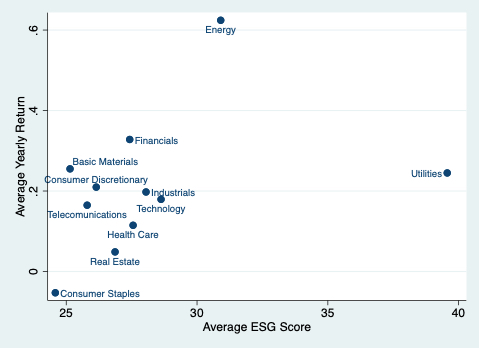
\includegraphics[scale=0.75]{Return_ESG.jpg}
%\end{figure}
%\FloatBarrier



% Uncomment this command to input a table
% Please add the following required packages to your document preamble:
% \usepackage{booktabs}

\end{document}

